\subsection{Admin System Overview}
\subsubsection{Class Diagram}

\begin{figure}[H]
    \centering
    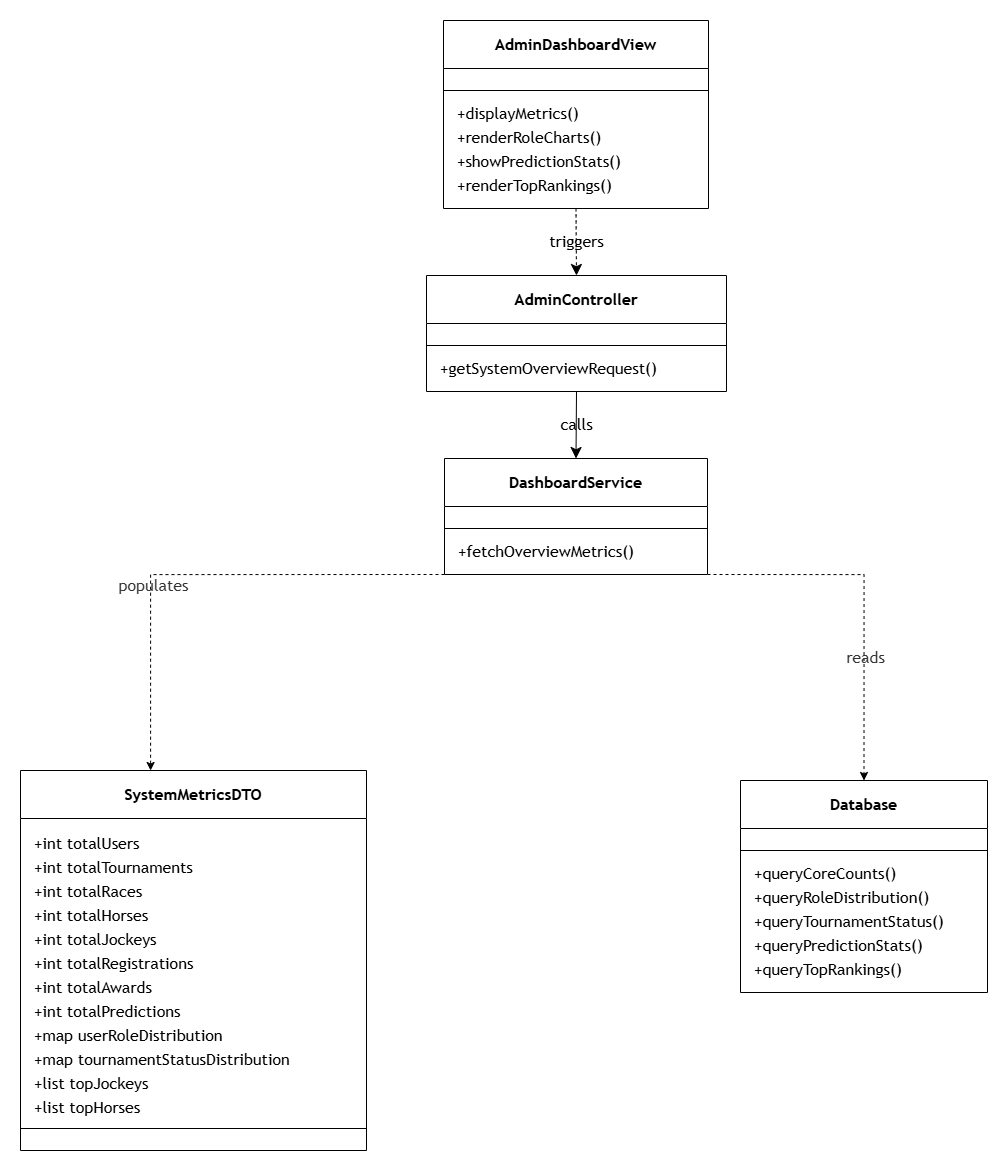
\includegraphics[width=\textwidth]{figures/design/admin/SystemOverview_ClassDiagram.png}
    \caption{Admin System Overview Class Diagram}
    \label{fig:admin_system_overview_class_diagram}
\end{figure}

\subsubsection{Sequence Diagram}

\begin{figure}[H]
    \centering
    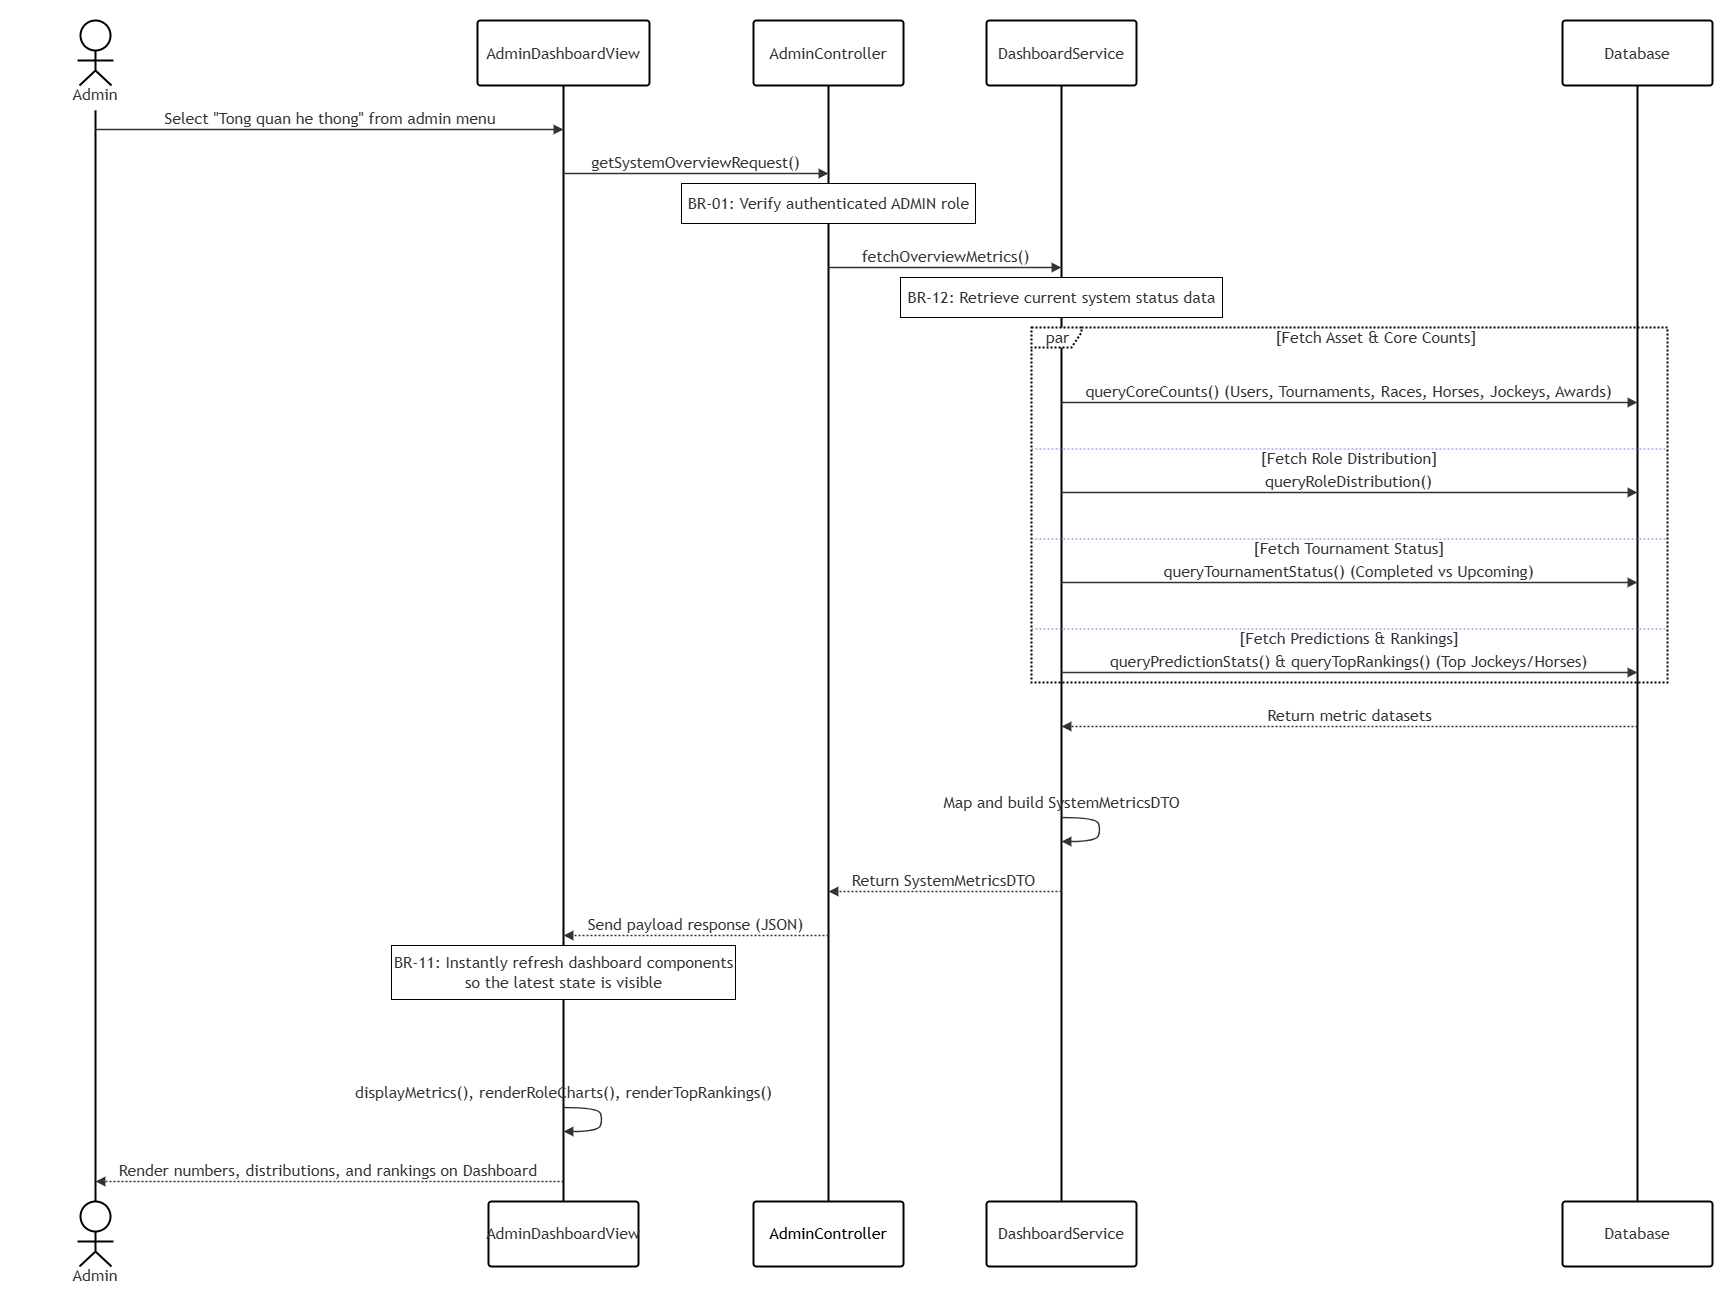
\includegraphics[width=\textwidth]{figures/design/admin/SystemOverview_SequenceDiagram.png}
    \caption{Admin System Overview Sequence Diagram}
    \label{fig:admin_system_overview_sequence_diagram}
\end{figure}

\subsubsection{Class Specification}

\begingroup
\small
\setlength{\tabcolsep}{3pt}
\TableStart{|>{\raggedright\arraybackslash}p{0.25\textwidth}|>{\raggedright\arraybackslash}p{0.31\textwidth}|>{\raggedright\arraybackslash}p{0.14\textwidth}|>{\raggedright\arraybackslash}p{0.25\textwidth}|}
\textbf{Class} & \textbf{Attributes / Methods} & \textbf{Type} & \textbf{Description} \\
\hline
AdminDashboard Router & get\_system\_overview() & controller / route & Handles HTTP GET requests to retrieve centralized analytics, validating BR-01 authorization. \\
\hline
SystemMetricsOut & total\_users, total\_tournaments, total\_races, total\_horses, total\_jockeys, total\_registrations, total\_awards, user\_roles, tournament\_status, top\_jockeys, top\_horses & DTO & Output data transfer object providing all aggregated dashboard numbers and top standings. \\
\hline
User & id, username, role, is\_active & entity & Database entity representing application users to fetch aggregate accounts and role groupings. \\
\hline
Tournament & id, name, status, start\_date, end\_date & entity & Database entity representing tournaments used to map status metrics. \\
\hline
Race & id, round\_id, status & entity & Database entity representing individual scheduled racing heats. \\
\hline
Registration & id, horse\_id, jockey\_id, status & entity & Database entity managing structural signups used to count processing assets. \\
\TableFinish{Admin System Overview class specification}{tab:admin_system_overview_class_spec}
\endgroup


\subsection{Admin Tournament Management}
\subsubsection{Class Diagram}

\begin{figure}[H]
    \centering
    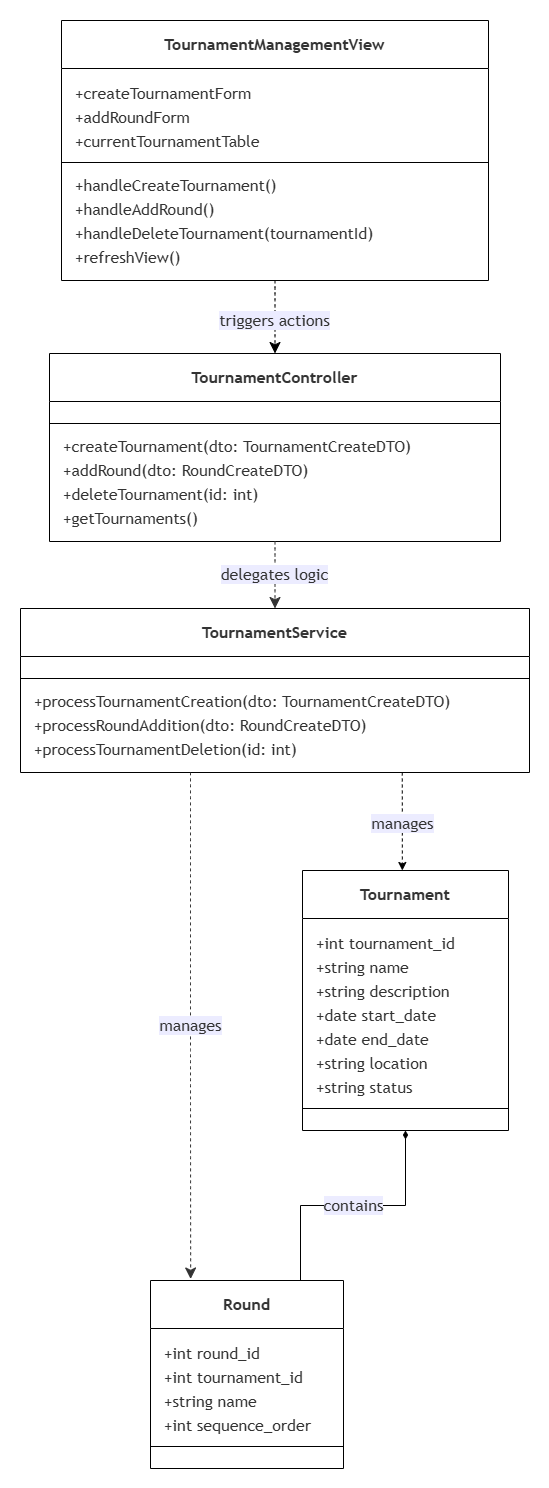
\includegraphics[
        width=\textwidth,
        height=0.85\textheight,
        keepaspectratio
    ]{figures/design/admin/TournamentManagement_ClassDiagram.png}
    \caption{Class Diagram for Tournament Management}
\end{figure}

\subsubsection{Sequence Diagram}

\begin{figure}[H]
    \centering
    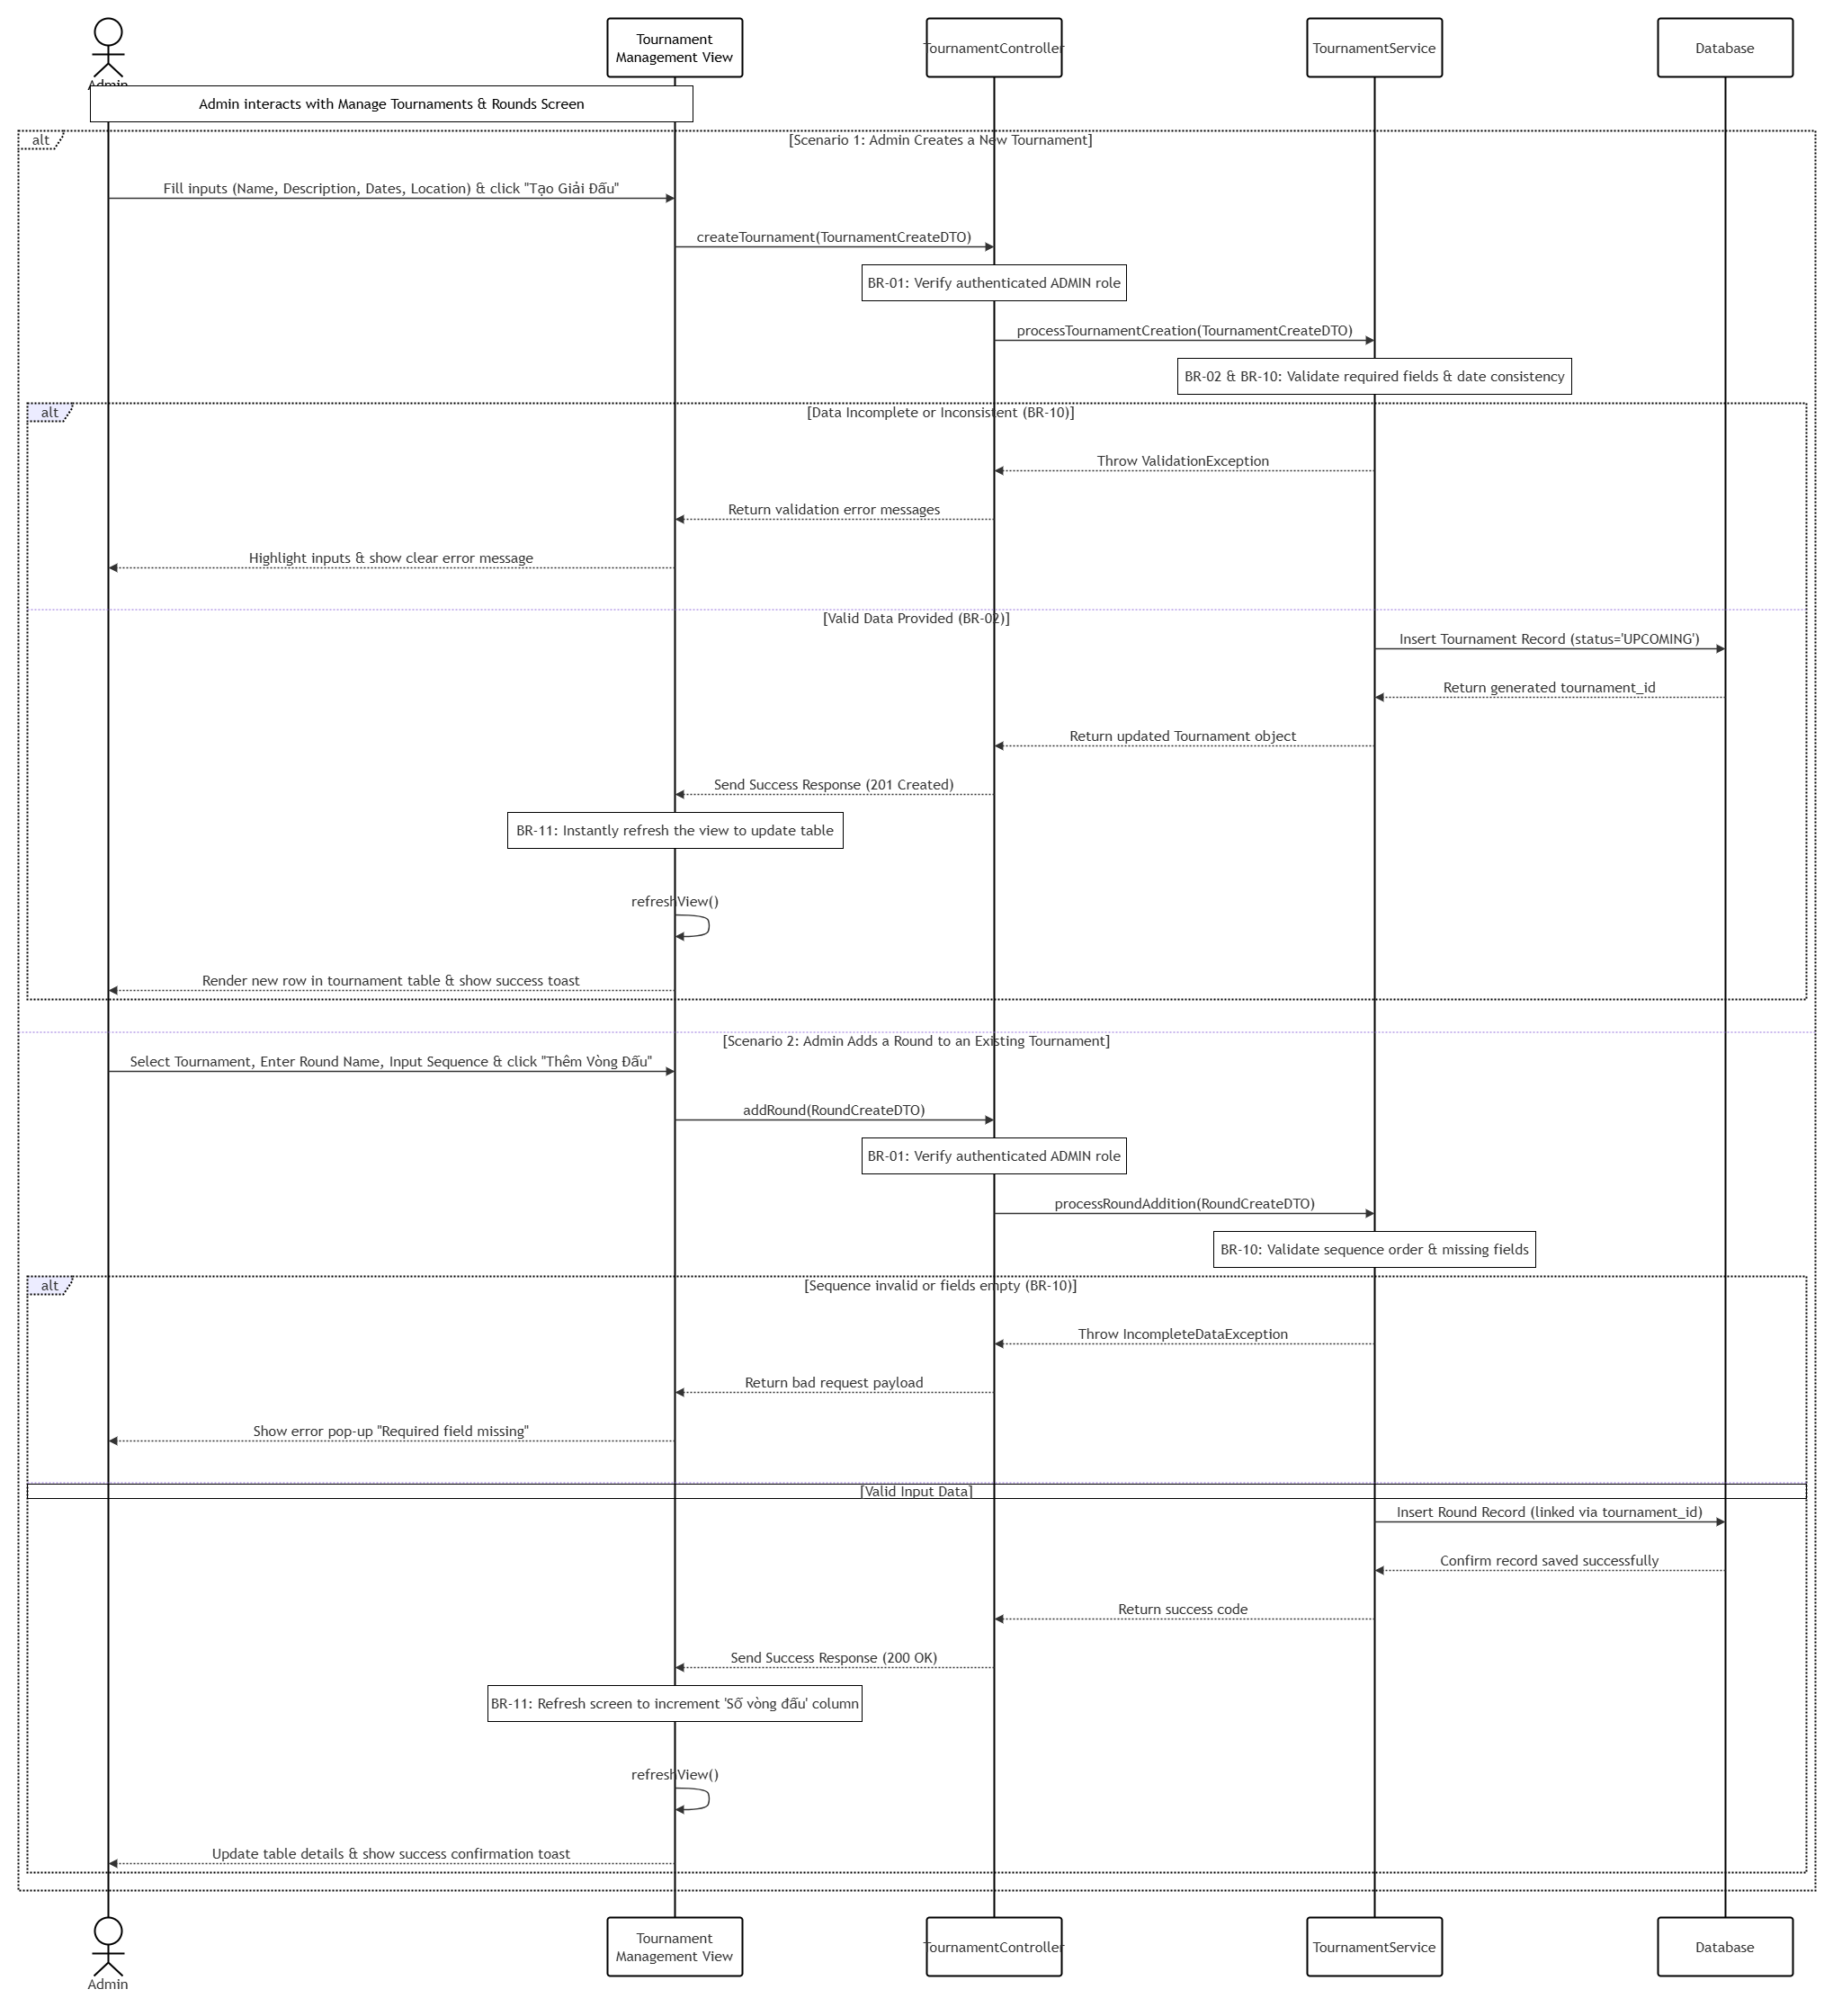
\includegraphics[width=\textwidth]{figures/design/admin/TournamentManagement_SequenceDiagram.png}
    \caption{Admin Tournament Management Sequence Diagram}
    \label{fig:admin_tournament_management_sequence_diagram}
\end{figure}

\subsubsection{Class Specification}

\begingroup
\small
\setlength{\tabcolsep}{3pt}
\TableStart{|>{\raggedright\arraybackslash}p{0.25\textwidth}|>{\raggedright\arraybackslash}p{0.31\textwidth}|>{\raggedright\arraybackslash}p{0.14\textwidth}|>{\raggedright\arraybackslash}p{0.25\textwidth}|}
\textbf{Class} & \textbf{Attributes / Methods} & \textbf{Type} & \textbf{Description} \\
\hline
TournamentRouter & create\_tournament(), add\_round(), get\_tournaments(), delete\_tournament() & controller / route & Handles administrative operations for structuring tournaments and competition stages. \\
\hline
TournamentCreate & name, description, start\_date, end\_date, location & DTO & Input data transfer object containing essential metrics to provision a new event profile. \\
\hline
RoundCreate & tournament\_id, name, sequence\_order & DTO & Input data transfer object configuring ordered stages inside a specific tournament context. \\
\hline
TournamentOut & id, name, description, start\_date, end\_date, location, status, round\_count & DTO & Output data transfer object supplying summary details of stored events. \\
\hline
Tournament & id, name, description, start\_date, end\_date, location, status & entity & Core domain entity storing structured racing tournament profile boundaries. \\
\hline
Round & id, tournament\_id, name, sequence\_order & entity & Database entity representing individual racing stages arranged sequentially. \\
\TableFinish{Admin Tournament Management class specification}{tab:admin_tournament_management_class_spec}
\endgroup

\subsection{Admin Registration Confirmation}
\subsubsection{Class Diagram}

\begin{figure}[H]
    \centering
    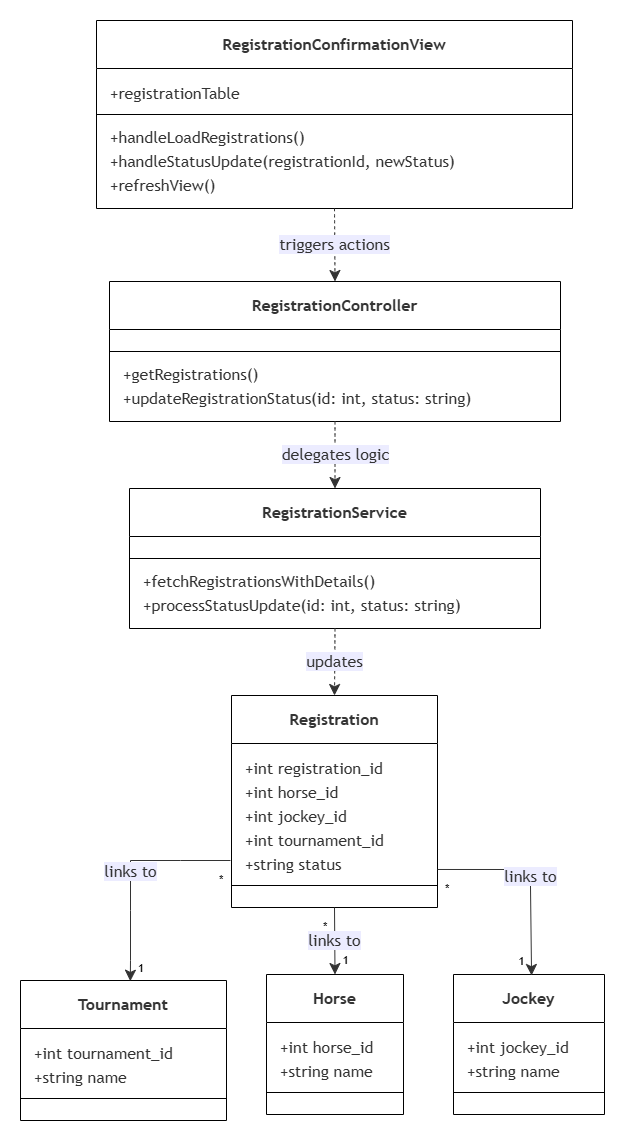
\includegraphics[
        width=\textwidth,
        height=0.85\textheight,
        keepaspectratio
    ]{figures/design/admin/Regis_Confirm_ClassDiagram.png}
    \caption{Class Diagram for Registration Confirmation}
\end{figure}

\subsubsection{Sequence Diagram}

\begin{figure}[H]
    \centering
    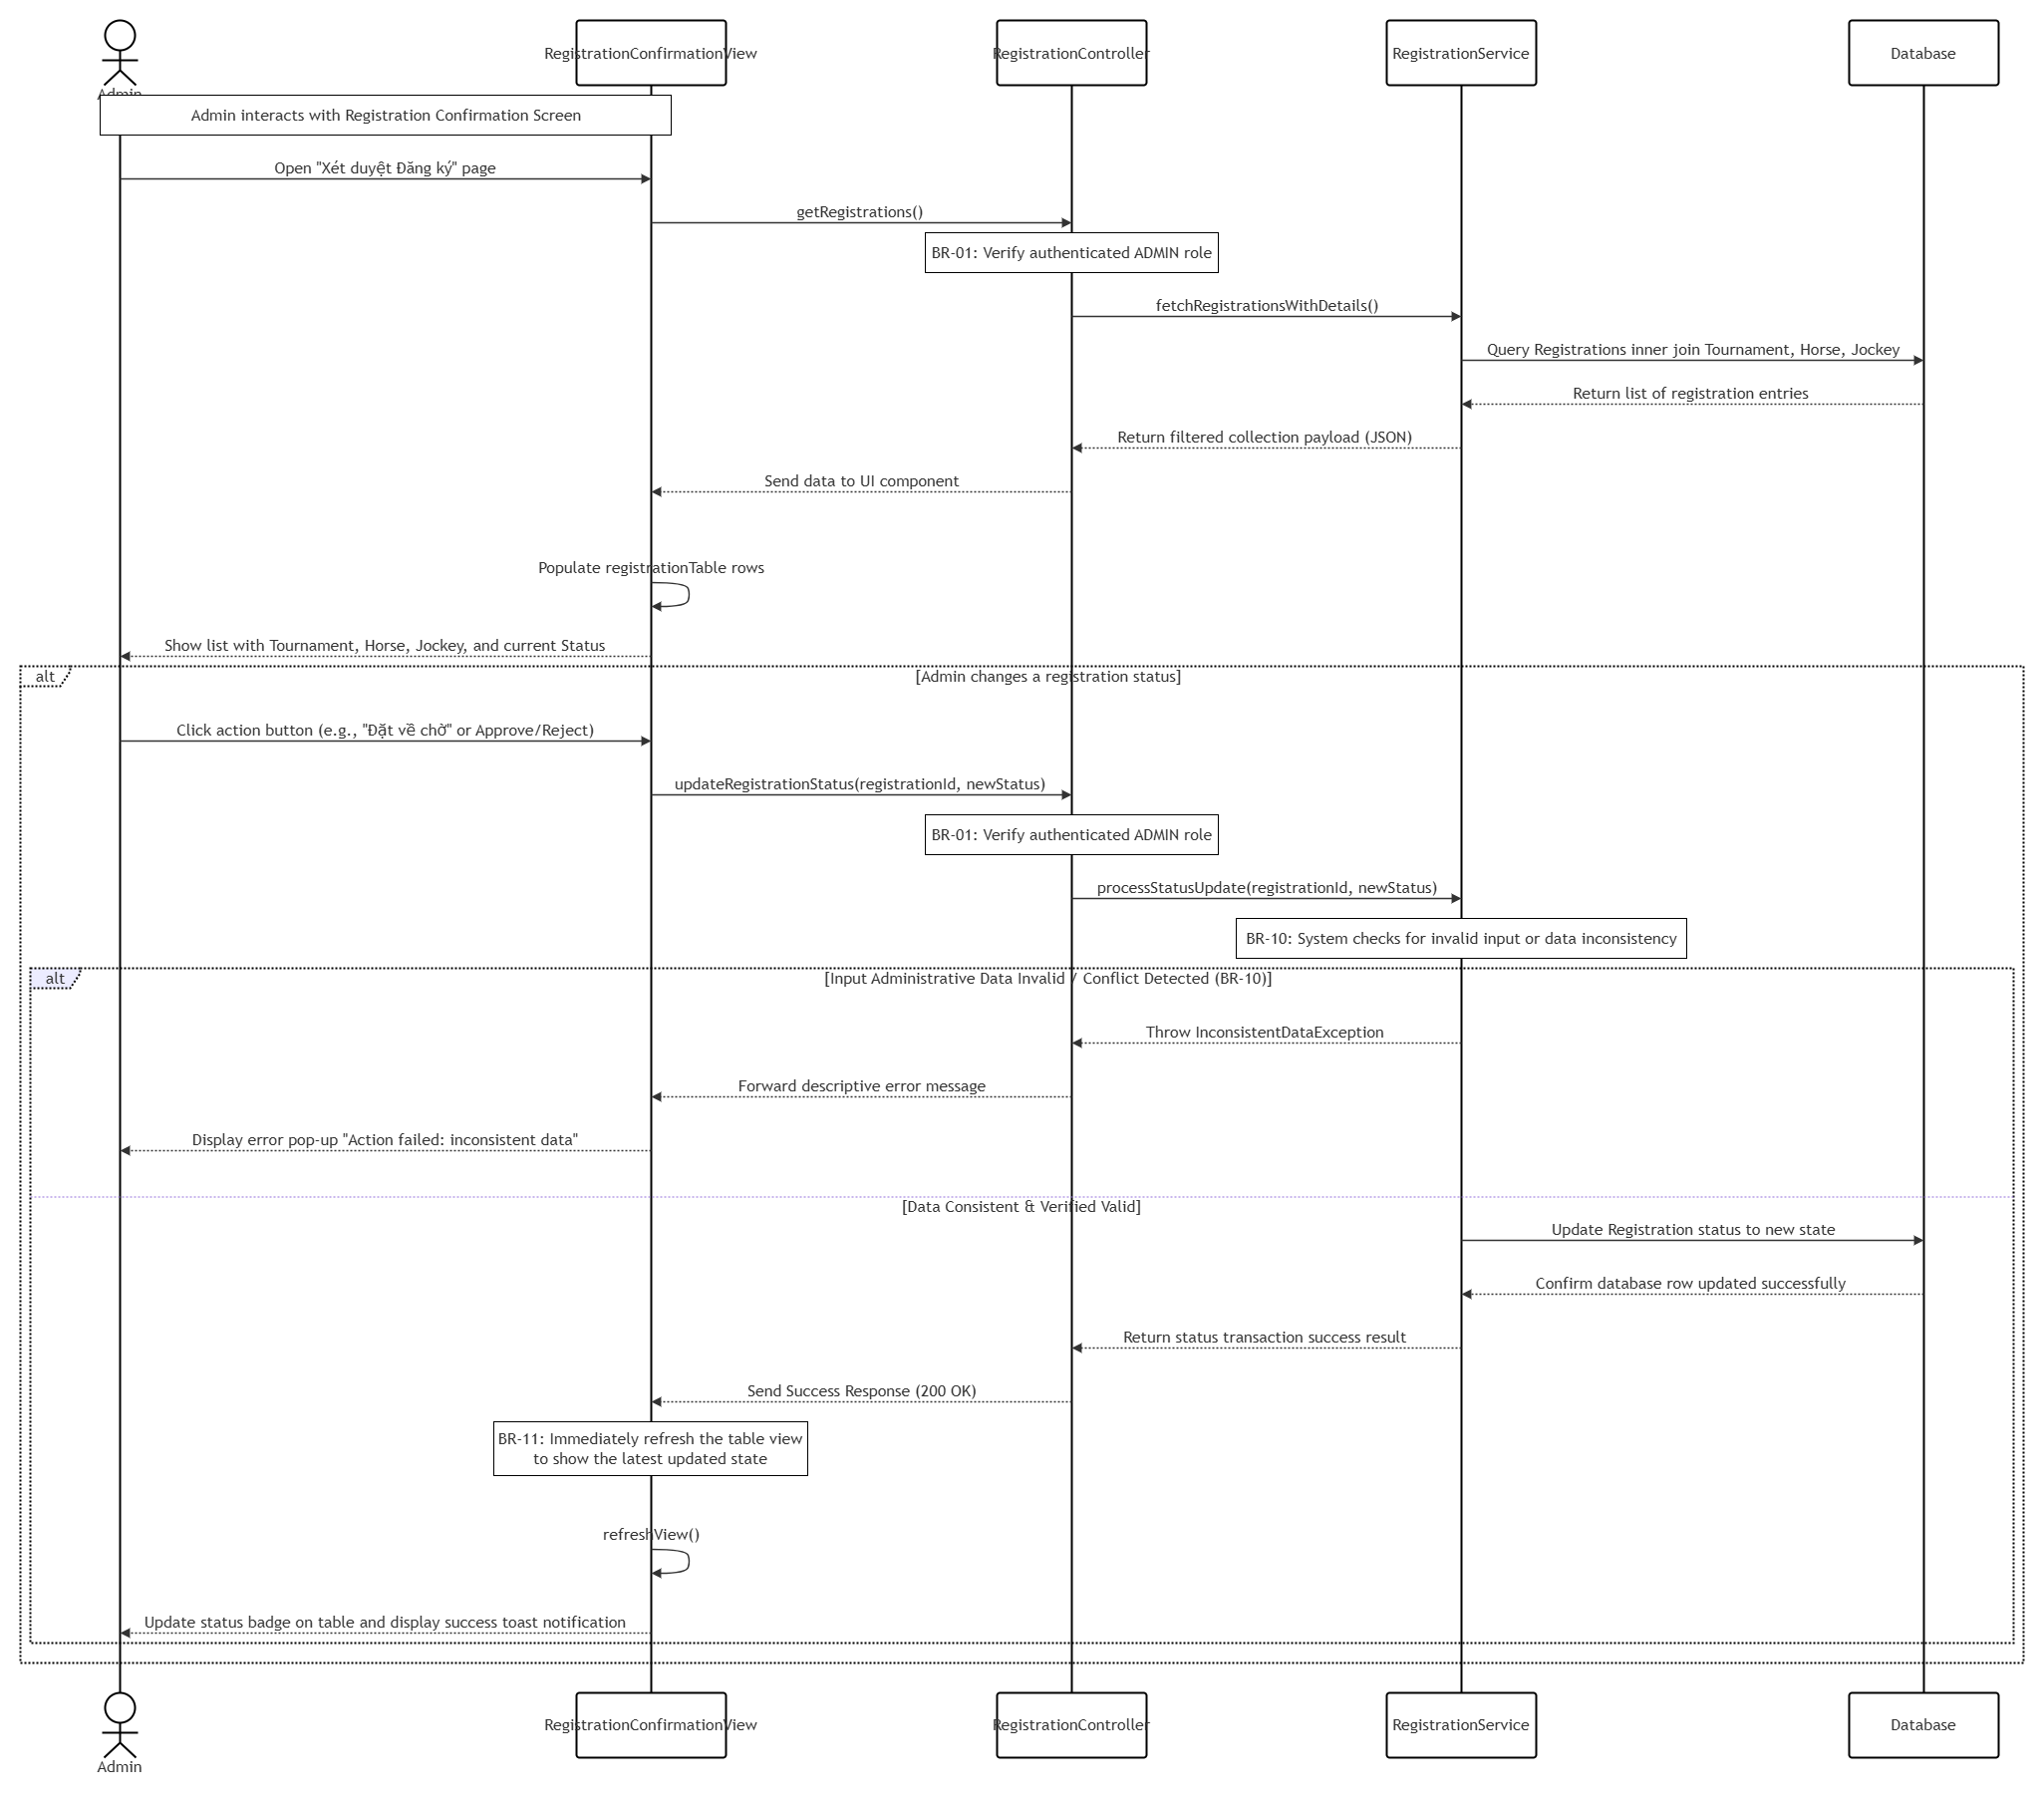
\includegraphics[width=\textwidth]{figures/design/admin/Regis_Confirm_SequenceDiagram.png}
    \caption{Admin Registration Confirmation Sequence Diagram}
    \label{fig:admin_registration_confirmation_sequence_diagram}
\end{figure}

\subsubsection{Class Specification}

\begingroup
\small
\setlength{\tabcolsep}{3pt}
\TableStart{|>{\raggedright\arraybackslash}p{0.25\textwidth}|>{\raggedright\arraybackslash}p{0.31\textwidth}|>{\raggedright\arraybackslash}p{0.14\textwidth}|>{\raggedright\arraybackslash}p{0.25\textwidth}|}
\textbf{Class} & \textbf{Attributes / Methods} & \textbf{Type} & \textbf{Description} \\
\hline
RegistrationRouter & get\_registrations(), update\_registration\_status() & controller / route & Exposes endpoints for loading applications and updating approval statuses. \\
\hline
RegistrationStatus Update & status & DTO & Input data transfer object carrying the updated status command (e.g., PENDING, APPROVED, REJECTED). \\
\hline
RegistrationDetailOut & id, tournament\_name, horse\_name, jockey\_name, status & DTO & Flattened output payload providing structural identities for administrative grid displays. \\
\hline
Registration & id, horse\_id, jockey\_id, tournament\_id, status & entity & Operational data entity containing processing records of team entries. \\
\hline
Horse & id, name & entity & Database entity providing naming contexts for registered horse components. \\
\hline
Jockey & id, name & entity & Database entity referencing profile information for underlying jockey entries. \\
\TableFinish{Admin Registration Confirmation class specification}{tab:admin_registration_confirmation_class_spec}
\endgroup
\subsection{Admin Schedule Races}
\subsubsection{Class Diagram}

\begin{figure}[H]
    \centering
    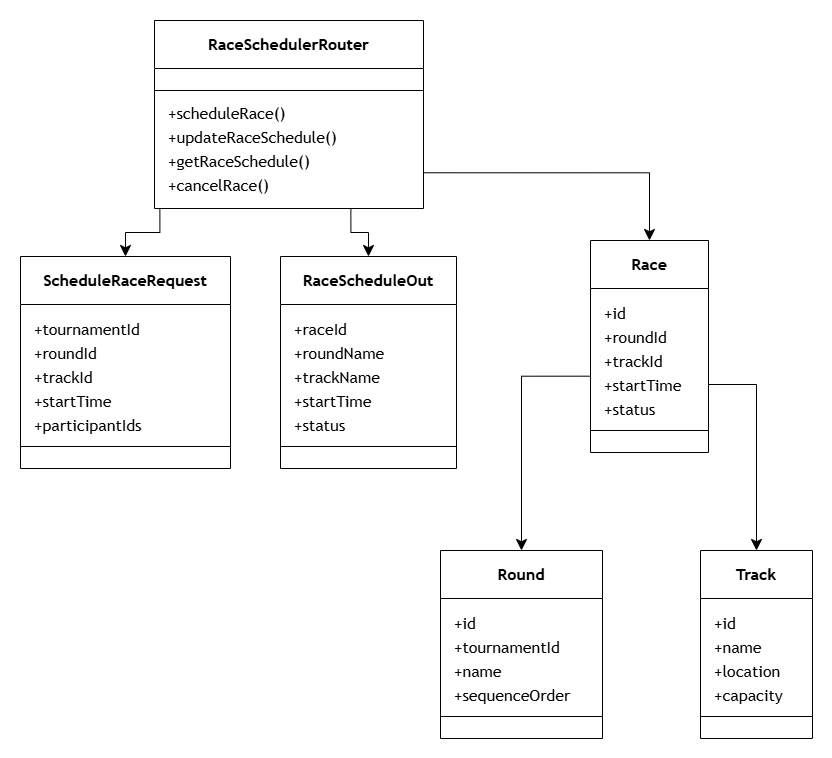
\includegraphics[width=\textwidth]{figures/design/admin/Schedule_Races_ClassDiagram.png}
    \caption{Class Diagram for Schedule Races}
    \label{fig:admin_schedule_races_class_diagram}
\end{figure}

\subsubsection{Sequence Diagram}

\begin{figure}[H]
    \centering
    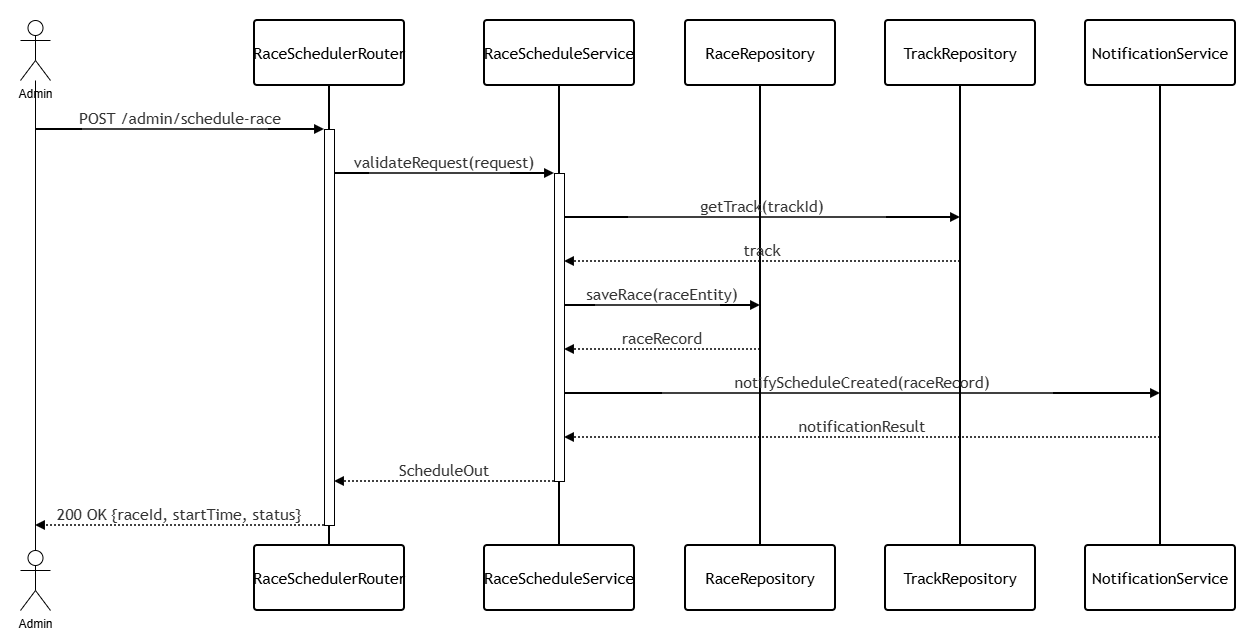
\includegraphics[width=\textwidth]{figures/design/admin/Schedule_Races_SequenceDiagram.png}
    \caption{Admin Schedule Races Sequence Diagram}
    \label{fig:admin_schedule_races_sequence_diagram}
\end{figure}

\subsubsection{Class Specification}

\begingroup
\small
\setlength{\tabcolsep}{3pt}
\TableStart{|>{\raggedright\arraybackslash}p{0.25\textwidth}|>{\raggedright\arraybackslash}p{0.31\textwidth}|>{\raggedright\arraybackslash}p{0.14\textwidth}|>{\raggedright\arraybackslash}p{0.25\textwidth}|}
\textbf{Class} & \textbf{Attributes / Methods} & \textbf{Type} & \textbf{Description} \\
\hline
RaceSchedulerRouter & schedule\_race(), update\_race(), get\_race\_schedule(), cancel\_race() & controller / route & Handles race scheduling operations and event lifecycle changes. \\
\hline
ScheduleRaceRequest & tournament\_id, round\_id, track\_id, start\_time, participant\_ids & DTO & Input DTO for creating or modifying a race schedule. \\
\hline
RaceScheduleOut & race\_id, round\_name, track\_name, start\_time, status, lane\_assignments & DTO & Output DTO delivering scheduled race details. \\
\hline
Race & id, round\_id, track\_id, start\_time, status, lane\_assignments & entity & Entity representing a scheduled race entry. \\
\hline
Round & id, tournament\_id, name, sequence\_order & entity & Entity representing a tournament round that contains races. \\
\hline
Track & id, name, location, capacity & entity & Entity representing a race track and its configuration. \\
\hline
Participant & id, horse\_id, jockey\_id, lane\_number & entity & Entity representing a horse-jockey entry assigned to a race lane. \\
\TableFinish{Admin Schedule Races class specification}{tab:admin_schedule_races_class_spec}
\endgroup

\subsection{Admin Manage Users}
\subsubsection{Class Diagram}

\begin{figure}[H]
    \centering
    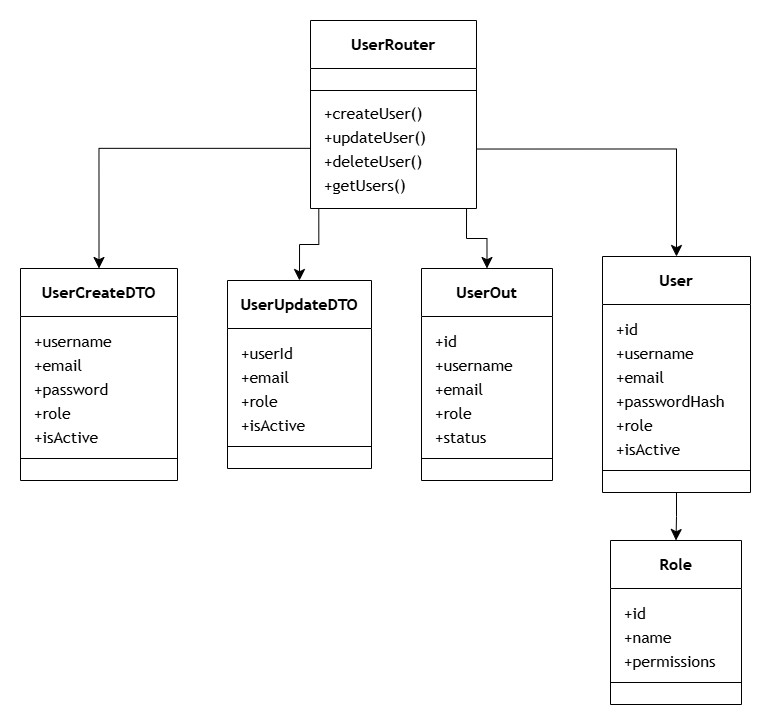
\includegraphics[width=\textwidth]{figures/design/admin/Manage_User_ClassDiagram.png}
    \caption{Class Diagram for Manage Users}
    \label{fig:admin_manage_users_class_diagram}
\end{figure}

\subsubsection{Sequence Diagram}

\begin{figure}[H]
    \centering
    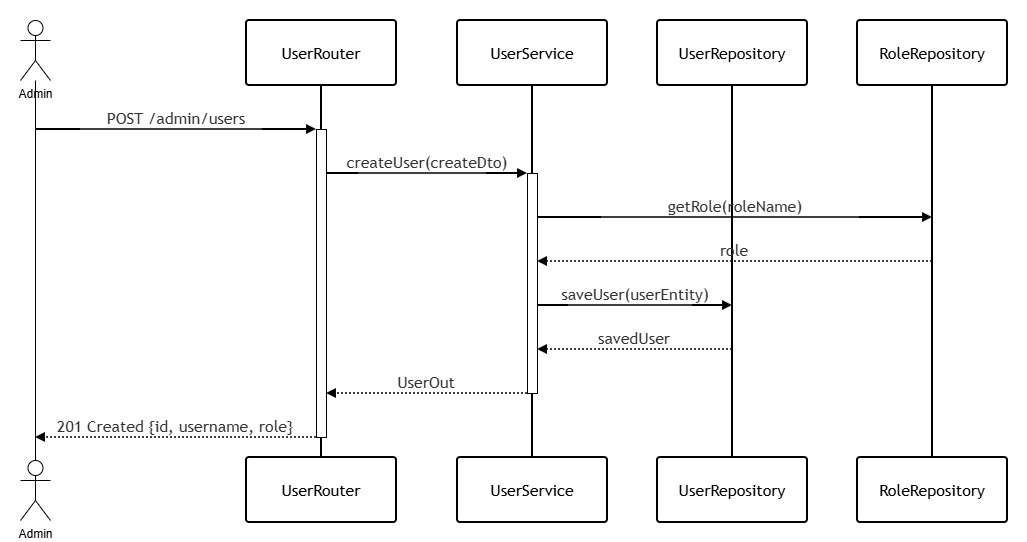
\includegraphics[width=\textwidth]{figures/design/admin/Manage_Users_SequenceDiagram.png}
    \caption{Admin Manage Users Sequence Diagram}
    \label{fig:admin_manage_users_sequence_diagram}
\end{figure}

\subsubsection{Class Specification}

\begingroup
\small
\setlength{\tabcolsep}{3pt}
\TableStart{|>{\raggedright\arraybackslash}p{0.25\textwidth}|>{\raggedright\arraybackslash}p{0.31\textwidth}|>{\raggedright\arraybackslash}p{0.14\textwidth}|>{\raggedright\arraybackslash}p{0.25\textwidth}|}
\textbf{Class} & \textbf{Attributes / Methods} & \textbf{Type} & \textbf{Description} \\
\hline
UserRouter & create\_user(), update\_user(), delete\_user(), get\_users() & controller / route & Manages user administration requests and account lifecycle actions. \\
\hline
UserCreate & username, email, password, role, is\_active & DTO & Input DTO used to create a new user account. \\
\hline
UserUpdate & user\_id, email, role, is\_active & DTO & Input DTO used to update user profile and status. \\
\hline
UserOut & id, username, email, role, status & DTO & Output DTO returning user details for display. \\
\hline
User & id, username, email, password\_hash, role, is\_active & entity & Entity storing user authentication and role data. \\
\hline
Role & id, name, permissions & entity & Entity representing role definitions and access permissions. \\
\TableFinish{Admin Manage Users class specification}{tab:admin_manage_users_class_spec}
\endgroup

\subsection{Admin Manage Rewards}
\subsubsection{Class Diagram}

\begin{figure}[H]
    \centering
    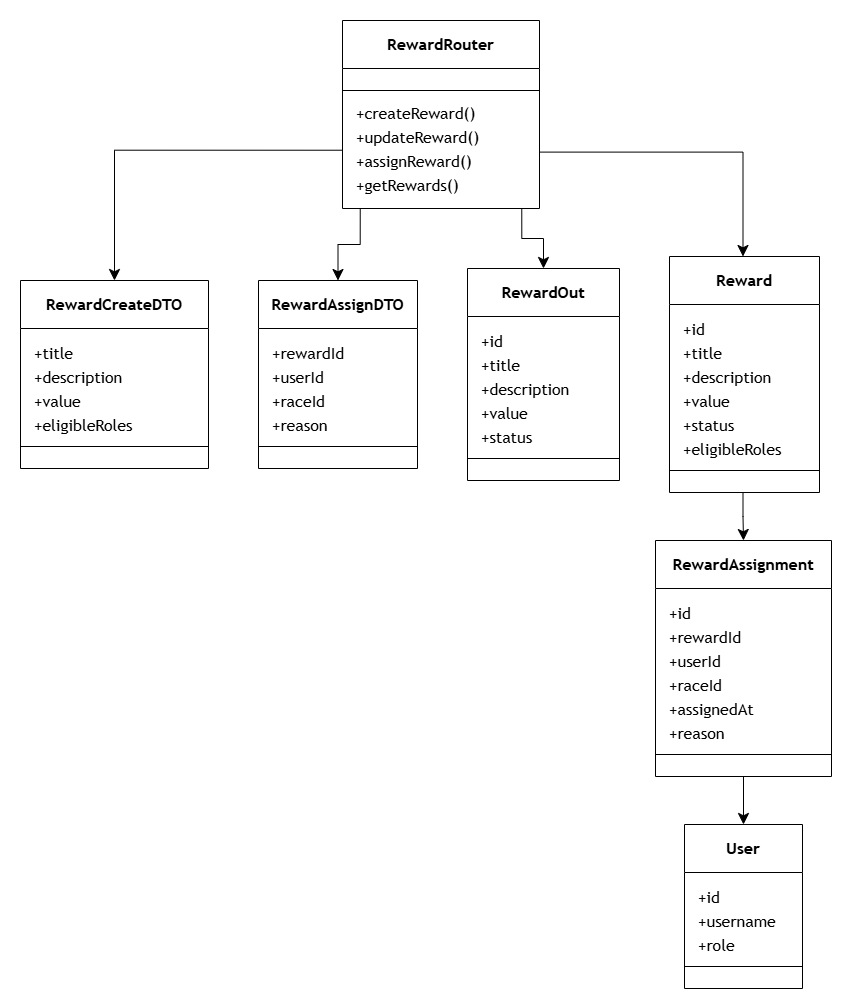
\includegraphics[width=\textwidth]{figures/design/admin/Manage_Rewards_ClassDiagram.png}
    \caption{Class Diagram for Manage Rewards}
    \label{fig:admin_manage_rewards_class_diagram}
\end{figure}

\subsubsection{Sequence Diagram}

\begin{figure}[H]
    \centering
    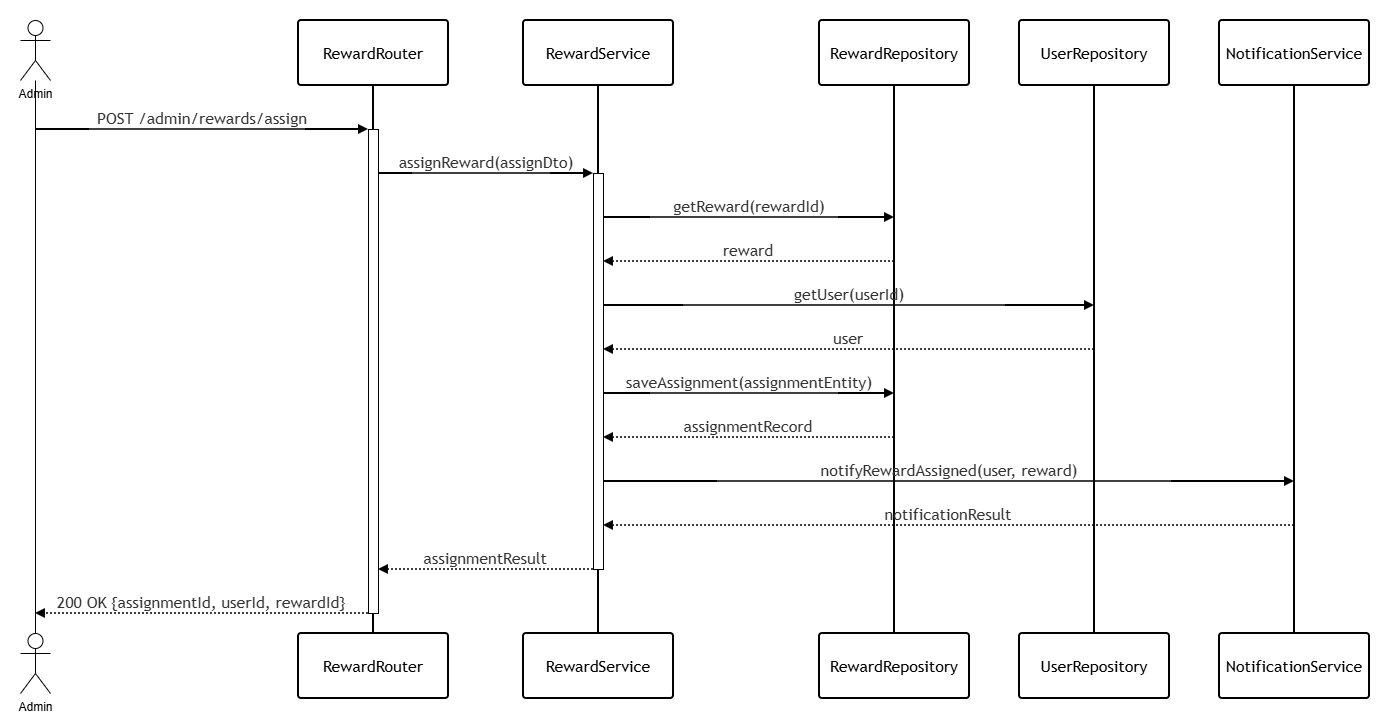
\includegraphics[width=\textwidth]{figures/design/admin/Manage_Rewards_SequenceDiagram.png}
    \caption{Admin Manage Rewards Sequence Diagram}
    \label{fig:admin_manage_rewards_sequence_diagram}
\end{figure}

\subsubsection{Class Specification}

\begingroup
\small
\setlength{\tabcolsep}{3pt}
\TableStart{|>{\raggedright\arraybackslash}p{0.25\textwidth}|>{\raggedright\arraybackslash}p{0.31\textwidth}|>{\raggedright\arraybackslash}p{0.14\textwidth}|>{\raggedright\arraybackslash}p{0.25\textwidth}|}
\textbf{Class} & \textbf{Attributes / Methods} & \textbf{Type} & \textbf{Description} \\
\hline
RewardRouter & create\_reward(), update\_reward(), assign\_reward(), get\_rewards() & controller / route & Manages reward configuration, assignment, and retrieval endpoints. \\
\hline
RewardCreate & title, description, value, rank, tournament\_id & DTO & Input DTO for defining a new reward within a tournament context. \\
\hline
RewardAssign & reward\_id, user\_id, race\_id, reason & DTO & Input DTO for assigning a reward to a user or race result. \\
\hline
RewardOut & id, title, description, value, rank, status & DTO & Output DTO returning reward information and distribution status. \\
\hline
Reward & id, title, description, value, rank, status, tournament\_id & entity & Entity representing a reward definition and its current state. \\
\hline
RewardAssignment & id, reward\_id, user\_id, race\_id, assigned\_at, reason & entity & Entity capturing reward assignment history and references. \\
\TableFinish{Admin Manage Rewards class specification}{tab:admin_manage_rewards_class_spec}
\endgroup